\section{Computational models for brain simulation}

The coupled differential equations that define a compartmental model of a
neuron can be solved numerically, and can therefore be programmed in a
high-level programming language relatively simply. However, while
programmatically solving differential equations is straightforward in principle,
the computational power and provision of memory required makes simulating large
networks of neurons difficult to do in practice \autocite{trappenberg_fundamentals_2009}.
Existing simulation packages provide a foundation from which biological
experiments can be conducted, and aim to abstract away purely computational
concerns. Some of these packages that have different approaches to solving this are described in more detail below. 

\subsection{Available neural simulation and modelling software packages}

\subsubsection{NEURON}
\begin{quote}
    NEURON is a simulation environment for developing and exercising models of
    neurons and networks of neurons. It is particularly well-suited to problems
    where cable properties of cells play an important role, possibly including
    extracellular potential close to the membrane), and where cell membrane
    properties are complex, involving many ion-specific channels, ion
    accumulation, and second messengers. It evolved from a long collaboration
    between Michael Hines and John W. Moore at the Department of Neurobiology,
    Duke University. Their express goal was to create a tool designed
    specifically for solving the equations that describe nerve cells.
\end{quote}
based on NEURON:
\autocite{hagen_lfpy_2019} \autocite{hagen_hybrid_2016}

\subsubsection{VERTEX}
The Virtual Electrode Recording Tool for EXtracellular potentials (VERTEX) is a
simulator for large networks of neurons written in the MATLAB programming
language. More specifically, it aims to reproduce the measurements that are
produced by in-vitro recordings from patients fitted with multi-electrode
arrays. This is achieved by locating each neuron in 3D space, placing virtual
electrodes in the same space, and calculating the change in potential at each
stage of the simulation at each electrode. The neuron model used in VERTEX is
also more advanced than similar models described in this section in that the
local field potential (LFP) of the neuron is spatially realistic \autocite{tomsett_virtual_2015}. A major
advantage of this design is that it becomes easy to map between general neuronal
activity in a simulated model and brain activity of, say, a real-world patient
in a medical trial. 

A 2019 update to VERTEX introduced a range of simulation features, the most
notable of which for the purposes of this project being Spike Time Dependant
Plasticity (STDP), which dynamically adapts the weighting of synapses based on
the observed causality of pre-synaptic spikes on post-synaptic spikes \autocite{thornton_virtual_2019}. Details
on how this may be implemented and used are covered further in Chapter 3.

\begin{figure}[h]
    \centering
    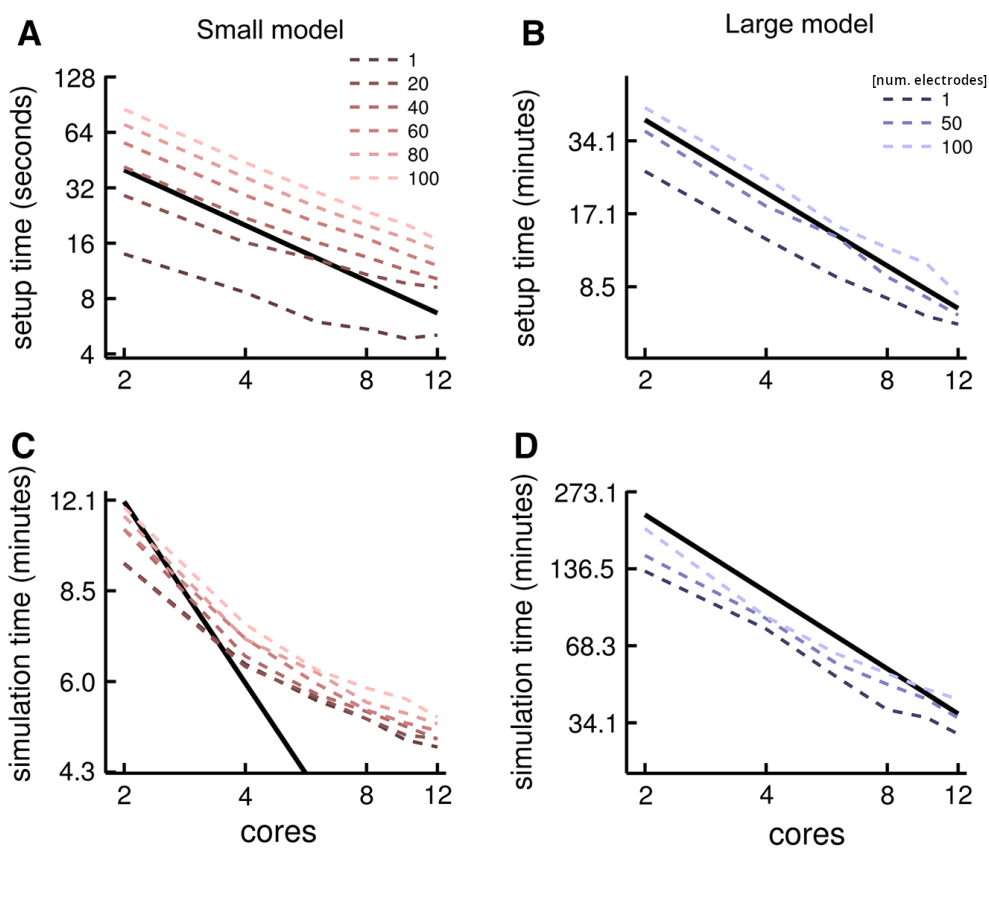
\includegraphics{figures/graphs/coresVERTEX.png}
    \DoubleCaption{Impact of parralel computation on simulation performance in VERTEX}
    {\cite{tomsett_virtual_2015}}
    \label{VERTEXparallel}
\end{figure}
\vspace{1ex}

VERTEX itself is multithreaded, and makes use of the compute pooling feature in
MATLAB to separate groups of tasks into separate logical threads. This means
that, with a sufficiently large model, doubling the number of available workers
in the pool nearly halves the time taken to simulate, as shown in figure
\ref{VERTEXparallel} above.

\subsubsection{BRIAN}
NEED A REFERENCE FOR BRIAN
\autocite{stimberg_brian_2019}

\subsection{Similarities in existing software packages}

Each of the mentioned software packages mentioned above is capable of doing XYZ,
but each has a distinct end goal. The VERTEX authors state that "QUOTE", while
BRIAN is designed less for a specific research purpose and more to be a
generally adoptable library for other developers and researchers to use in their
own projects. The LFPy authors have taken a combined approach, with thorough
documentation of the project, but the tool is still understandably designed for
the research purposes of its authors. 